\newpage
%\section{Background Theory}
\chapter{Background Theory}
\label{sec:theory}

\section{Anomaly detection}
The process of detecting anomalies in a hyperspectral image is called anomaly detection. For a spectral vector to be considered as an anomaly, it has to be significantly different to its neighboring background. Four issues arising in anomaly detection \cite{chang2006characterization} is:
\\
 
\begin{itemize}
  \item Q1: How large for a target to be considered as an anomaly?
  \item Q2: How does an anomaly respond to its neighbouring pixels?
  \item Q3: How sensitive is anomaly detection to noise?
  \item Q4: How are different anomalies to be detected and classified?
\end{itemize}

The above-mentioned issues are important for the choice of anomaly detection algorithm, and will be further discussed in this chapter.
\\
Algorithms used for anomaly detection outputs the probability that the spectral pixel vector is an anomaly. A higher output indicates a higher probability for the pixel vector being an anomaly.
%\subsection{Background compression}
% See book

%\subsection{Causality}

\subsection{Reed-Xiaoli algorithm}
The Reed-Xiaoli(RX) algorithm \cite{reed1990adaptive} is one of the most widely used algorithms for anomaly detection in HSI, and is considered as the benchmark anomaly detection algorithm for hyperspectral data \cite{yang2015dual}.  
\\
The RX algorithm was developed to address the scenario where no prior knowledge about the target signatures is available. Assuming that a single pixel target, \textbf{x}, is the observation test vector, the result of the RX algorithm is given by the filter in equation \ref{eq:RX_algorithm}.

\begin{equation}
    RX(\textbf{x}) = (\textbf{x} - \textbf{u}_b)^T \sum^{-1} (\textbf{x} - \textbf{u}_b)	
\label{eq:RX_algorithm}
\end{equation}

In equation \ref{eq:RX_algorithm} $\textbf{u}_b$ is the estimated background clutter sample mean, computed from the set of all pixel vectors in the image (referred to as the \textit{global set}  ). $\sum$ is the estimated background clutter covariance, estimated on the global set. Since the covariance is computed on the global set of pixels, the HSI needs to collect all data contained in the entire image before the RX anomaly detector(AD) can start. This means that the RX-algorithm in the original variant does not have the possibility to operate in real-time. 

\subsection{Local RX algorithm}
An often used and important variant of the RX algorithm is the local RX(LRX) algorithm. By substituting the sample covariance matrix computed on the global set with the correlation matrix computed on a kernel of size $k x k$ pixel vectors, it is possible to increase the parallelism of the AD and to get near real-time performance. The LRX can be considered as a local AD because each pixel of the image has its own correlation matrix. This correlation matrix is computed on the square kernel of size $k x k$. The result of the LRX AD can then be expressed as in equation \ref{eq:LRX}. $\textbf{x}$ is the observation test pixel vector. $\textbf{R}$$_{k x k}$$(\textbf{x})}$ is the correlation matrix of pixel vector $\textbf{x}$ computed on a square kernel of size $k x k$ containing local neighbouring pixels. See figure \ref{fig:LRX}. 

\begin{equation}
    \delta_k^{LRX}(\textbf{x}) = \textbf{x}^T\textbf{R}_{k x k}(\textbf{x})^{-1}\textbf{x}
    \label{eq:LRX}
\end{equation}


\begin{figure}[H]
\centering
   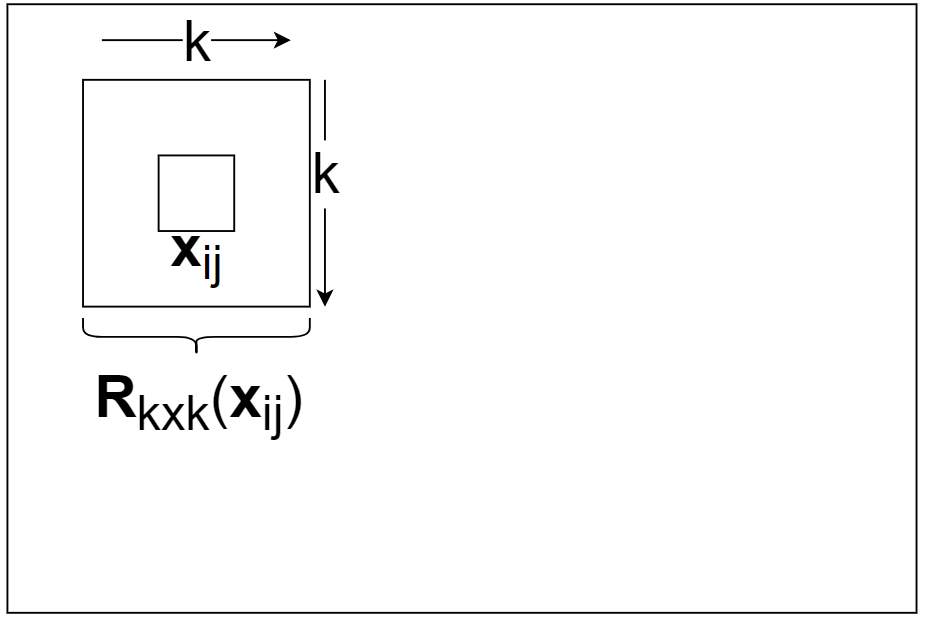
\includegraphics[scale=0.3]{images/LRX.PNG}
  \caption{ Visualization of a kernel of size $k x k$ used in LRX. } 
  \label{fig:LRX}
\end{figure}


\section{Adaptive Causal Anomaly Detection}
An improved variant of the RX AD is the Adaptive Causal Anomaly detection (ACAD) \cite{chang2006characterization}. One issue of the RX algorithm is that previously detected anomalies with strong spectral signatures may have an impact upon the detection of later anomalies. This is shown in \cite{chang2006characterization}. ACAD is adaptive in the way that it builds a map of detected anomalies, and removes the previously detected anomaly pixel vectors from the causal sample correlation set. \\
Another benefit of ACAD relative to RX and LRX is that it is real-time. This is achieved by using the causal correlation matrix $\textbf{R}$($\textbf{x}$), defined in equation \ref{eq:caus_corr}, instead of the covariance or the correlation matrix computed on the global or a local set of pixel vectors, as in RX and LRX, respectively. In equation \ref{eq:caus_corr} $\textbf{x}$ is the observation test pixel vector, and $k$ is the index of the pixel vector currently being processed. The sum in equation \ref{eq:caus_corr} sums the correlation matrix for the pixel sample vectors {$\textbf{x}_1$, ....$\textbf{x}_k$}.  

\begin{equation}
    \textbf{R}(\textbf{x}_k)=\frac{1}{k}\sum_{i=1}^k\textbf{x}_i\textbf{x}_i^T
    \label{eq:caus_corr}
\end{equation}

To remove the previously detected anomalous pixel vectors from the correlation set, the sample spectral correlation matrix, referred to as causal anomaly-removed sample spectral correlation matrix, is presented in equation \ref{eq:caus_corr_anomaly_removed} \cite{chang2006characterization}.

\begin{equation}
    \Tilde{\textbf{R}}(\textbf{x}_k)= \textbf{R}(\textbf{x}_k) - \sum_{t_j\in\Delta(k)}\textbf{t}_j\textbf{t}_j^T
    \label{eq:caus_corr_anomaly_removed}
\end{equation}

In equation \ref{eq:caus_corr_anomaly_removed} $\Delta(k)$ is the set of all earlier detected anomalous pixel vectors $\textbf{t}_j$ prior to the image pixel currently being processed, $\textbf{x}_k$.
\\
ACAD can then be defined as in equation \ref{eq:ACAD}.
\begin{equation}
    \delta^{ACAD}(\textbf{x}_k)= \textbf{x}_k^T\Tilde{\textbf{R}}^{-1}(\textbf{x}_k)\textbf{x}_k
    \label{eq:ACAD}
\end{equation}

ACAD is a causal filter, meaning that only the pixels previosly processed are used for anomaly detection.  It computes the correlation matrix for the previously captured pixel sample vector {$\textbf{x}_1$, ....$\textbf{x}_k$} up to the pixel currently being processed, $k$, as shown in equation \ref{eq:caus_corr}. This means that ACAD might be implemented in real-time and near-real time, seeing as pixels can be processed as soon as they are captured by the push-broom HSI and the AD does not need to wait for the entire image to be loaded into memory. \\

An anomalous pixel vector have a significant spectral vector difference from its surroundings. Since ACAD is causal, the surroundings is defined as the $n_{acad}$ previously processed pixels. %To evaluate if a spectral vector is anomalous,
ACAD defines the variable $u_k$, shown in equation \ref{eq:u_k}. $u_k$ is used to be able to evaluate if a pixel vector is anomalous. 

\begin{equation}
    u_k = \frac{1}{n_{acad}}\sum_{i-1}^{n_{acad}}  \delta^{ACAD}(\textbf{x}_{k-i})
    \label{eq:u_k}
\end{equation}

In order to classify if a pixel vector is anomalous or not, the variable $t_k$ is introduced, defined in equation \ref{eq:t_k}. If $t_k$ is greater than a predetermined value $\tau$, the pixel vector is considered an anomaly an added to the set of anomalous targets. If not, it is used in subsequent data processing. 

\begin{equation}
    t_k = \delta^{ACAD}(\textbf{x}_{k}) - u_k
    \label{eq:t_k}
\end{equation}


The four issues labelled Q1, Q2, Q3 and Q4 still remains. 

\subsenction{Q1 ACAD}



%Problem RX; If an earlier detected anomaly has a strong signature, it may have significant impact on detection of subsqeunt detected anomalies later. Solves by removing anomalies detected from the set R when calculating the correlation matrix.\\
%Another issue arising in K-AD(RXD) is that the size of anomaloies to be detected cannot be too large. HOw large can the size be to be considered an anomaly? - Obviously, a data sample vector that can be identified visually generally should not be considered as an anomaly. Beta; rate of image size to the size of an anomaly. Empirically \approx 100\\

%Third issue ; how close is too close for two anomalies to be detected as two separate anomalies?
%\\
%Fourth issue; How to distinguish two detected anomalies from one another.
\\ 
%Benefits ACAD: \\
%- ACAD builds and updates an anomaly library and generates an anomaly map to provide spatial coordinates of all its detected anomalies in the original image. This anomaly map can also be used to classify all the detected anomalies. \\
%- ACAD can be considered to be real time, even though the data processing may take time. Once the processing of data is completed, the whole process of anomaly dettection is also completed at nearly the same time. 
%\\
%This implies that the performance of ACAD is not determined by the relative size of the entire image to the anomaly, but rather by the number of data sample vectors considered in $n_{acad}$.

%\\ Question
%\\ Causality; in causality, will the first pixel-vector processed have a high probability of being detected as a anomality?\\
%-Yes, might be an issue. Remedied by the ACAD according to the book.

%Note to self; include comparison here of the different Anomalies Detector



\section{Inverse matrix}
Doing the inverse of a matrix is computationally intensive. There exists multiple algorithms for computing the matrix inverse. One option is to use QR-decompostion.  

\subsection{QR-Factor}

A QR-decomposition can certainly be used for matrix inversion because if A=QR then A−1=R−1Q−1=R−1QT and R−1 is easy to compute because R is triangular.\\
Q-factor
• Q is m × n with orthonormal columns (QTQ = I)
• if A is square (m = n), then Q is orthogonal (Q^TQ = QQ^T = I)
R-factor
• R is n × n, upper triangular, with nonzero diagonal elements
• R is nonsingular (diagonal elements are nonzero)

\subsubsection{Givens rotation}

Givens rotation can create an upper triangular matrix

